\chapter{\difficult{Higher-dimensional Algebra}}\label{chapter:hda}

    The main reference for this chapter is the series of papers carrying the same name by \textit{Baez et al} \cite{HDA5, HDA6}. For Kapranov-Voevodsky 2-vector spaces we also refer to the original paper \cite{kapranov_voevodsky}. For fusion and modular categories the main reference is \cite{etingof}.

\section{Graded vector spaces}\label{section:graded_spaces}

    Similar to definition \ref{group:graded_ring} we can define a graded object in the category of vector spaces:
    \newdef{Graded vector space}{\index{degree}\index{graded!vector space}\label{linalgebra:graded_vector_space}
        Consider an index set $I$ (finite or countable) and let $V_i$ be a vector space for all $i\in I$. The vector space
        \begin{gather}
            V = \bigoplus_{i\in I}V_i
        \end{gather}
        is called a graded vector space (with grading $I$). The index $i$ is often called the \textbf{degree} of the subspace $V_i$ in $V$.
    }
    \newdef{Finite type}{\index{finite!type}
        A graded vector space is said to be of finite type if it is finite-dimensional in each degree.
    }

    \newdef{Graded algebra}{\index{graded!algebra}
        Let $V$ be a graded vector space with the additional structure of an algebra given by the multiplication $\star$. Then $V$ is a graded algebra if $\star$ maps $V_k\times V_l$ to $V_{k+l}$.
    }
    \newdef{Graded commutativity}{\index{graded!commutativity}\label{linalgebra:graded_commutative}
        A graded algebra $V$ is said to be graded-commutative if we have
        \begin{gather}
            v\star w = (-1)^{\deg(v)\deg(w)}w\star v
        \end{gather}
        for all homogeneous elements $v,w\in V$.
    }

    \newdef{Super vector space}{\index{super!vector space}\label{linalgebra:superspace}
        A $\mathbb{Z}_2$-graded vector space.
    }

    \begin{example}[Superalgebra]\index{super!algebra}\label{linalgebra:superalgebra}
        A $\mathbb{Z}_2$-graded algebra, i.e. there exists a decomposition
        \begin{gather}
            A = A_0\oplus A_1
        \end{gather}
        such that for all $i,j\mod 2$:
        \begin{gather}
            A_i\star A_j \subseteq A_{i+j}.
        \end{gather}
    \end{example}

    \newdef{Parity functor}{\index{parity}
        Consider the category $\mathbf{sVect}$ of super vector spaces. We can define the parity functor $\func{\Pi}{sVect}{sVect}$ as the functor which interchanges even and odd subspaces:
        \begin{align}
            (\Pi V)_0 &:= V_1\\
            (\Pi V)_1 &:= V_0.
        \end{align}
    }
    \newdef{Symmetric tensors}{
        Using the parity functor one can write the exterior algebra\footnote{See definition \ref{tensor:exterior_algebra}.} $\Lambda^\bullet(V)$ as the symmetric algebra $\text{Sym}^\bullet(\Pi V)$. In a similar way one can write the symmetric algebra on a super vector space $V=V_0\oplus V_1$ as \[\text{Sym}^n(V)=\bigoplus_{p+q=n}\text{Sym}^p(V_0)\otimes\Lambda^q(V_1).\]
    }

    \newdef{Differential graded algebra}{\index{dg-algebra}\label{linalgebra:dg_algebra}
        \nomenclature[A_DGA]{dga}{differential graded algebra}
        A differential graded algebra (often denoted by \textbf{dg-algebra} or even \textbf{dga}) is a graded algebra equipped with a differential of degree 1 (see definition \ref{homalg:chain_complex}).\footnote{In the homological convention we use a morphism of degree $-1$.}
    }
    \newdef{Semifree dga}{\index{semifree}
        A dga is said to be semifree if the underlying graded algebra is isomorphic (as a graded algebra) to the tensor algebra of a graded vector space.
    }
    \newdef{Differential graded-commutative algebra}{
        \nomenclature[A_DGCA]{dgca}{differential graded-commutative algebra}
        A graded-commutative differential graded algebra. This is often abbreviated as \textbf{dgca}.
    }
    \newdef{Semifree dgca}{
        A dgca is said to be semifree if the underlying graded-commutative algebra is isomorphic (as a graded-commutative algebra) to the Grassmann algebra over some graded vector space.
    }

\subsection{Supermatrices}

    For this section we will relax the requirement that we are working over a field $K$, instead we will be working over a supercommutative ring. This means that we will be working with (graded) modules instead of true vector spaces.

    \newdef{Supermatrix}{\index{parity}
        Every linear transformation between super vector spaces $(V_0, V_1)$ and $(W_0, W_1)$ can be decomposed as the sum of 4 linear transformations between the even/odd subspaces:
        \begin{itemize}
            \item $A:V_0\rightarrow W_0$,
            \item $B:V_1\rightarrow W_0$,
            \item $C:V_0\rightarrow W_1$, and
            \item $D:V_1\rightarrow W_1$.
        \end{itemize}
        If we represent these transformations as matrices, then the full transformation can be represented as a block matrix \[X=\begin{pmatrix}A&B\\C&D\end{pmatrix}\] where we used the same notation to denote the matrices associated to the linear transformations.

        These matrices can be decomposed according to their \textbf{parity}. Not all supermatrices preserve the grading, or equivalently, not all linear transformations of super vector spaces are morphisms of super vector spaces. The ones that are, are said to have even parity and they are of the form \[X=\begin{pmatrix}\text{even}&\text{odd}\\\text{odd}&\text{even}\end{pmatrix}\] where by even/odd we mean that the entries in these blocks have even/odd parity as elements of the underlying (graded) ring. It should be clear that these matrices indeed preserve the grading, since acting with an odd scalar on an odd vector gives an even vector (and similar for the other combinations). The matrices that do not preserve the grading are said to have odd parity and are of the form \[X=\begin{pmatrix}\text{odd}&\text{even}\\\text{even}&\text{odd}\end{pmatrix}.\]
    }

    \newdef{Supertrace}{\index{trace}
        The supertrace of a supermatrix generalizes the trace of an ordinary matrix. Given the block matrix form from the previous definition we define the supertrace as follows:
        \begin{gather}
            \text{str}(X) = \text{tr}(A)-\text{tr}(D).
        \end{gather}
    }
    \begin{property}
        As was the case for the ordinary trace, the supertrace is invariant under basis transformations. Furthermore, the cyclicity property also still holds if we modify it slightly as to be compatible with the grading:
        \begin{gather}
            \text{str}(XY) = (-1)^{|X||Y|}\text{str}(YX)
        \end{gather}
        where $|X|, |Y|$ denote the parities of the supermatrices.
    \end{property}

    \newdef{Berezinian}{\label{linalgebra:berezinian}
        The Berezinian or \textbf{superdeterminant} generalizes the determinant of an ordinary matrix. It is (uniquely) defined through the following two conditions:
        \begin{enumerate}
            \item $\text{Ber}(XY) = \text{Ber}(X)\text{Ber}(Y)$, and
            \item $\text{Ber}(e^X) = e^{\text{str}(X)}$.
        \end{enumerate}
        An explicit formula is given by
        \begin{gather}
            \text{Ber}(X) = \det(A - BD^{-1}C)\det(D)^{-1}.
        \end{gather}
        It should be noted that the Berezinian is only well-defined for invertible even matrices.
    }

\subsection{Lie superalgebras}

    \newdef{Internal Lie algebra}{\index{Lie!algebra}
        Let $(\textbf{C}, \otimes, \mathbf{1})$ be a linear symmetric monoidal category with braiding $\sigma$. A Lie algebra internal to \textbf{C} is an object $A\in\ob{C}$ and a morphism \[[\cdot, \cdot]:A\otimes A\rightarrow A\] satisyfing the following conditions:
        \begin{enumerate}
            \item \textbf{Antisymmetry}: $[\cdot, \cdot] + [\cdot, \cdot]\circ\sigma_{A, A} = 0$, and
            \item \textbf{Jacobi identity}: $[\cdot, [\cdot, \cdot]] + [\cdot, [\cdot, \cdot]]\circ\tau + [\cdot, [\cdot, \cdot]]\circ\tau^2= 0$
        \end{enumerate}
        where $\tau = (\mathbbm{1}\otimes\sigma_{A, A})\circ(\sigma_{A, A}\otimes\mathbbm{1})$ denotes cyclic permutation.
    }
    \begin{example}[Lie superalgebra]
        If we use the braiding $\sigma(a\otimes b) = (-1)^{\deg(a)\deg(b)}b\otimes a$ in the category \textbf{sVect}, we obtain the notion of a Lie superalgebra (also called a super Lie algebra).
    \end{example}
    \begin{example}[dg-Lie algebras]
        Lie algebras internal to $\mathbf{Ch}_\bullet(\mathbf{Vect})$ (or its generalization to graded vector spaces) are called dg-Lie algebras. Sometimes these are also called strict $L_\infty$-algebras (see further below).
    \end{example}

\section{Monoidal categories II: Duality}\label{section:duality}

    \newdef{Dual object}{\index{dual!object}\label{cat:dual}
        Let $(\mathbf{C}, \otimes, \mathbf{1})$ be a monoidal category and let $A\in\ob{C}$. A left dual\footnote{Analogously, $A$ is called the \textbf{right dual} of $A^*$. The right dual of $B$ is often denoted by $^*B$.} $A^*$ of $A$ is an object in $\mathbf{C}$ together with two morphisms $\eta:\mathbf{1}\rightarrow A\otimes A^*$ and $\varepsilon:A^*\otimes A\rightarrow\mathbf{1}$, called the \textbf{unit} and \textbf{counit} morphisms\footnote{Also called the \textbf{coevaluation} and \textbf{evaluation} morphisms.}, such that the diagrams \ref{fig:dual_object1} and \ref{fig:dual_object2} commute. $A$ is said to be \textbf{dualizable} if the object $A^*$ and the morphisms $\eta,\varepsilon$ exist.

        \begin{figure}[ht!]
            \centering
            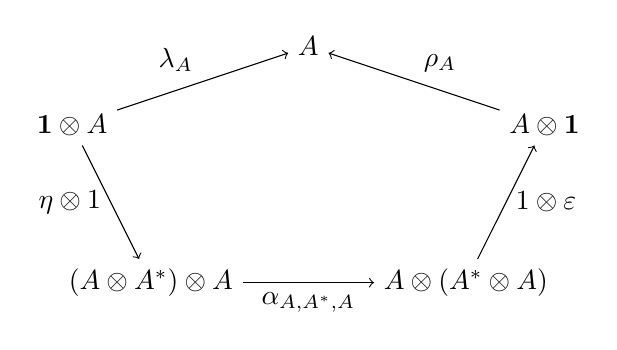
\begin{tikzpicture}
                \node (A) at (0, 0) {$A$};
                \node (1A) at (-3, -1) {$\mathbf{1}\otimes A$};
                \node (A1) at (3, -1) {$A\otimes\mathbf{1}$};
                \node (1AAA) at (-2, -3) {$(A\otimes A^*)\otimes A$};
                \node (AAA1) at (2, -3) {$A\otimes(A^*\otimes A)$};
                \draw[->] (1A) -- node[above left]{$\lambda_A$} (A);
                \draw[->] (A1) -- node[above right]{$\rho_A$} (A);
                \draw[->] (1A) -- node[left]{$\eta\otimes\mathbbm{1}$} (1AAA);
                \draw[->] (AAA1) -- node[right]{$\mathbbm{1}\otimes\varepsilon$} (A1);
                \draw[->] (1AAA) -- node[below]{$\alpha_{A, A^*, A}$} (AAA1);
            \end{tikzpicture}
            \caption{Dual object I.}
            \label{fig:dual_object1}
        \end{figure}
        \begin{figure}[ht!]
            \centering
            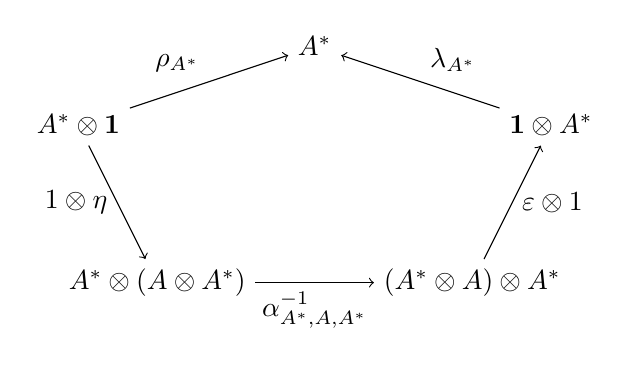
\begin{tikzpicture}
                \node (A) at (0, 0) {$A^*$};
                \node (A1) at (-3, -1) {$A^*\otimes\mathbf{1}$};
                \node (1A) at (3, -1) {$\mathbf{1}\otimes A^*$};
                \node (AAA1) at (-2, -3) {$A^*\otimes(A\otimes A^*)$};
                \node (1AAA) at (2, -3) {$(A^*\otimes A)\otimes A^*$};
                \draw[->] (A1) -- node[above left]{$\rho_{A^*}$} (A);
                \draw[->] (1A) -- node[above right]{$\lambda_{A^*}$} (A);
                \draw[->] (A1) -- node[left]{$\mathbbm{1}\otimes\eta$} (AAA1);
                \draw[->] (1AAA) -- node[right]{$\varepsilon\otimes\mathbbm{1}$} (1A);
                \draw[->] (AAA1) -- node[below]{$\alpha^{-1}_{A^*, A, A^*}$} (1AAA);
            \end{tikzpicture}
            \caption{Dual object II.}
            \label{fig:dual_object2}
        \end{figure}
    }

    \newdef{Rigid category\footnotemark}{\index{category!rigid}\index{category!autonomous}
        \footnotetext{Also called an \textbf{autonomous category}.}
        A monoidal category in which all duals exist. If only left (resp. right) duals exist then the category is said to be left (resp. right) rigid.
    }

    \begin{property}[Braided categories]\label{cat:braided_rigid}
        In general it is not true that left and right duals coincide, however in a braided monoidal category this is the case.
    \end{property}
    \newdef{Compact closed category}{\index{category!compact closed}
        A symmetric rigid category is also called a compact closed category.
    }

    \begin{example}[FinVect]\index{dual!space}\index{resolution!of the identity}
        Consider the category $\mathbf{FinVect}$ of finite-dimensional vector spaces (we assume the ground field to be $\mathbb{R}$). The categorical dual of a vector space $V$ is the algebraic dual $V^*$. The unit morphism is given by the ''resolution of the identity'':
        \begin{gather}
            \eta: \mathbf{1}\rightarrow V\otimes V^*:1\mapsto\sum_{i=1}^{\dim(V)}e_i\otimes \phi^i
        \end{gather}
        where $\{e_i\}$ and $\{\phi^i\}$ are bases of $V$ and $V^*$ respectively.

        It should be noted that the category $\mathbf{Vect}$ of all vector spaces is not rigid. By property \ref{cat:braided_rigid} above, left and right duals coincide in any braided monoidal category (such as $\mathbf{Vect}$). However for infinite-dimensional vector spaces it is known that $A\cong(A^*)^*$ never holds and as such the rigidity cannot be extended to $\mathbf{Vect}$.
    \end{example}
    \begin{property}[Tannaka duality]\index{Tannaka duality}
        Let us again consider the category $\mathcal{V}=\mathbf{FinVect}_K$ where we now explicitly mention the underlying ground field. Using coends one can reconstruct the base field from its modules, i.e. the objects in $\mathcal{V}$:\footnote{This result can be shown to hold for all compact closed categories $\mathcal{V}$. In this context it is known as \textbf{Tannaka reconstruction}.}
        \begin{gather}
            \int^{V\in\mathcal{V}}V^*\otimes V\cong K.
        \end{gather}
        A more general statement goes as follows:
        \begin{gather}
            \int^{V\in\mathcal{V}}\mathcal{V}(V, -)\otimes\text{id}_{\mathcal{V}}V\cong\text{id}_{\mathcal{V}}.
        \end{gather}
        The components $\eta_V:\mathcal{V}(V, V)\rightarrow K$ of the coend can be shown to coincide with the trace and such the trace obtains a universal property.
    \end{property}
    \remark{This property can also be generalized by replacing $\mathcal{V}$ by a category $\mathbf{Mod}_A$ for some finite-dimensional algebra $A$. The end and coend than give respectively the algebra $A$ and its dual $A^*$.}

    The trace on $\mathbf{FinVect}$ can be generalized as follows:
    \newdef{Trace}{\index{trace}
        Let $(\mathbf{C}, \otimes, \mathbf{1})$ be a rigid category and let $f\in\hom_{\mathbf{C}}(A, A^{**})$. The left (\textbf{categorical} or \textbf{quantum}) trace of $f$ is defined as the following morphism in End$_{\mathbf{C}}(\mathbf{1})$:
        \begin{gather}
            \text{tr}^L(f):=\varepsilon_{A^*}\circ(f\otimes\mathbbm{1})\circ\eta_A.
        \end{gather}
        If $f\in\hom_{\mathbf{C}}(A, ^{**}A)$ then the right trace is defined similarly:
        \begin{gather}
            \text{tr}^R(f):=\varepsilon_{^{**}A}\circ(\mathbbm{1}\otimes f)\circ\eta_{^*A}.
        \end{gather}
    }
    \begin{property}
        The following linear algebra-like properties hold for the categorical trace:
        \begin{itemize}
            \item $\text{tr}^L(f) = \text{tr}^R(f^*)$,
            \item $\text{tr}^L(f\otimes g) = \text{tr}^L(f)\text{tr}^L(g)$, and
            \item For additive categories: $\text{tr}^L(f\oplus g) = \text{tr}^L(f) + \text{tr}^L(g)$.
        \end{itemize}
        The second and third property can be stated analogously for the right trace.
    \end{property}

    \newdef{Pivotal category}{\index{pivotal structure}
        Let $\mathbf{C}$ be a rigid monoidal category. A pivotal structure on $\mathbf{C}$ is a monoidal natural isomorphism $a_A:A\cong A^{**}$.
    }

    \newdef{Dimension}{\index{dimension}
        Let $(\mathbf{C}, a)$ be a pivotal category and consider an object $V\in\ob{C}$. The dimension of $V$ is defined as follows:
        \begin{gather}
            \label{category:pivotal_dimension}
            \dim_a(V) := \text{tr}^L(a_V).
        \end{gather}
    }

    \newdef{Spherical category}{\index{spherical structure}
        Let $(\mathbf{C}, a)$ be a pivotal category. If the left and right traces (with respect to $a$) coincide in $\mathbf{C}$, i.e. $\dim_a(V) = \dim_a(V^*)$, then the pivotal structure is said to be spherical.
    }

    \newdef{Symmetric monoidal dagger category}{\index{category!dagger}
        A symmetric monoidal category $(\mathbf{C},\otimes,\mathbf{1})$ which also carries the structure of a dagger category \ref{cat:dagger_category} such that
        \begin{gather}
            (f\otimes g)^\dag = f^\dag\otimes g^\dag
        \end{gather}
        and such that the coherence and braiding morphisms are unitary.
    }
    \newdef{Dagger-compact category}{
        A symmetric monoidal dagger category which is also a compact closed category such that the following diagram commutes:
        \begin{gather*}
            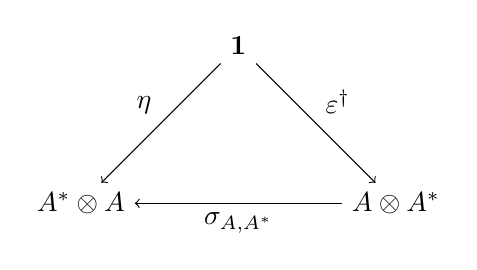
\begin{tikzpicture}
                \node (1) at (0, 0) {$\mathbf{1}$};
                \node (A*A) at (-2, -2) {$A^*\otimes A$};
                \node (AA*) at (2, -2) {$A\otimes A^*$};
                \draw[->] (1) -- node[above left]{$\eta$} (A*A);
                \draw[->] (1) -- node[above right]{$\varepsilon^\dagger$} (AA*);
                \draw[<-] (A*A) -- node[below]{$\sigma_{A,A^*}$} (AA*);
            \end{tikzpicture}
        \end{gather*}
    }

\section{Tensor and fusion categories}

    Some definitions might slightly differ from the ones in the main reference and some properties might be stated less generally. By $k$ we will mean an algebraically closed field (often this will be $\mathbb{C}$).

    \newdef{Tensor category}{\index{tensor!category}
        A monoidal category with the following properties:
        \begin{enumerate}
            \item it is rigid,
            \item it is Abelian,
            \item it is $k$-linear (and it is so in a way compatible with the Abelian structure),
            \item $\text{End}(\mathbf{1})\cong k$, and
            \item $-\otimes -$ is bilinear on morphisms.
        \end{enumerate}
        Some authors (such as \cite{etingof}) also add ''locally finite'' as a condition (see definition \ref{category:locally_finite}).
    }
    \remark{If $k$ is not algebraically closed one should exchange the last condition by the condition that $\mathbf{1}$ is a simple object. However, if $k$ is algebraically closed then these statements are equivalent.}

    \newdef{Pointed tensor category}{\index{pointed!tensor category}
        A tensor category is said to be pointed if all of its simple objects are (weakly) invertible.
    }

    \newdef{Fusion category}{\index{fusion!category}
        A semisimple finite tensor category.
    }

    \begin{property}
        Let $\mathbf{M}$ be a fusion category. There exists a natural isomorphism $X\cong X^{**}$.
    \end{property}

    \sremark{Although any fusion category admits a natural isomorphism between an object and its double dual, this morphism does not need to be monoidal. The fact that all fusion categories are pivotal was conjectured by Etingof, Ostrik and Nikshych. Currently the best one can do for a general fusion category is a monoidal natural transformation between the identity functor and the fourth dualization functor $X\cong X^{****}$.}

    \newdef{Categorical dimension}{\index{dimension}
        Consider a fusion category $\mathbf{M}$ and choose a natural isomorphism $a:\text{id}_{\mathbf{M}}\xrightarrow{\ \sim\ }\ast\ast$. For every simple object $X$ one can define a dimension function, sometimes called the \textbf{norm squared}, in the following way:
        \begin{gather}
            |X|^2 = \text{tr}(a_X)\text{tr}((a_X^{-1})^*).
        \end{gather}
        If $\mathbf{M}$ is pivotal then this becomes $|X|^2 = \dim_a(X)\dim_a(X^*)$. In particular, when $\mathbf{M}$ is spherical, this becomes $|X|^2 = \dim_a(X)^2$.

        The categorical dimension\footnote{Sometimes called the \textbf{M\"uger dimension}.} is then defined as follows:
        \begin{gather}
            \dim(\mathbf{M}) = \sum_{X\in\mathcal{O}(\mathbf{M})}|X|^2
        \end{gather}
        where $\mathcal{O}(\mathbf{M})$ denotes the set of isomorphism classes of simple objects.
    }
    \remark{It should be noted that the above quantities do not depend on the choice of isomorphism $a_X:X\cong X^{**}$ since all of them only differ by a scale factor.}
    \begin{property}
        For any fusion category $\mathbf{M}$ one has that $\dim(\mathbf{M})\neq 0$. In particular, if $k=\mathbb{C}$ then $\dim(\mathbf{M})\geq1$ (since the norm squared of any simple object is then also positive).
    \end{property}

    \newdef{$G$-graded fusion category}{\index{G!grading}
        A semisimple linear category $\mathbf{C}$ is said to have a \textbf{$G$-grading}, where $G$ is a finite group, if it can be decomposed as follows:
        \begin{gather}
            \mathbf{C} \cong \bigoplus_{g\in G} \mathbf{C}_g
        \end{gather}
        where every $\mathbf{C}_g$ is again linear and semisimple. A fusion category $\mathbf{C}$ is said to be a ($G$-)graded fusion category if it admits a $G$-grading such that the tensor product functor maps $\mathbf{C}_g\times\mathbf{C}_h$ into $\mathbf{C}_{gh}$.
    }

    \begin{example}[$G$-graded vector spaces]\label{category:g_graded}
        Define the category $\mathbf{Vect}_G^\omega$ as having the same objects and morphisms as $\mathbf{Vect}_G$ (the category of $G$-graded vector spaces) but with the associator given by the the 3-cocycle $\omega\in H^3(G; k^\times)$.
    \end{example}
    \begin{property}
        Any pointed fusion category is equivalent to a category of the form $\mathbf{Vect}_G^\omega$ for some $G$ and $\omega\in H^3(G; k^\times)$.
    \end{property}

    \begin{theorem}[Tannaka duality]\index{Tannaka duality}
        The representation category of a weak Hopf algebra has the structure of a fusion category. Conversely, any fusion category can be obtained as the representation category of a weak Hopf algebra.
    \end{theorem}

\section{Ribbon and modular categories}

    \newdef{Ribbon structure}{
        Consider a braided monoidal category $(\mathbf{M}, \otimes, \mathbf{1})$ with braiding $\sigma$. A \textbf{twist} or \textbf{balancing} is a natural transformation $\theta$ such that the following equation is satisfied for all $X, Y\in\ob{M}$:
        \begin{gather}
            \theta_{X\otimes Y} = (\theta_X\otimes\theta_Y)\circ\sigma_{Y, X}\circ\sigma_{X, Y}.
        \end{gather}
        If in addition $\mathbf{M}$ is rigid and the twist satisfies $\theta_{X^*} = (\theta_X)^*$ for all $X\in\ob{M}$ then one speaks of a ribbon category.
    }

    \newdef{Drinfeld morphism}{
        Let $(\mathbf{M}, \otimes, \mathbf{1})$ be a rigid braided monoidal category with braiding $\sigma$. This structure admits a canonical natural isomorphism $X\cong X^{**}$ defined as follows:
        \begin{gather}
            X\xrightarrow{\mathbbm{1}_X\otimes\eta_{X^*}}X\otimes X^*\otimes X^{**}\xrightarrow{\sigma_{X, X^*}\otimes\mathbbm{1}_{X^{**}}}X^*\otimes X\otimes X^{**}\xrightarrow{\varepsilon_X\otimes\mathbbm{1}_{X^{**}}}X^{**}.
        \end{gather}
    }
    \begin{property}
        Let $\mathbf{M}$ be a braided monoidal category. Consider the canonical natural isomorphism $u_X:X\cong X^{**}$ defined above. Any natural isomorphism $\psi_X:X\cong X^{**}$ can be written as $u_X\theta_X$ where $\theta\in\text{Aut}(\mathbbm{1}_{\mathbf{M}})$. It is not hard to see that this natural isomorphism is monoidal (hence pivotal) exactly when $\theta$ is a twist. If $\mathbf{M}$ is a fusion category then the pivotal structure is spherical if and only if $\theta$ gives a ribbon structure.
    \end{property}

    \newdef{Premodular category}{
        A ribbon fusion category. Equivalently, a spherical braided fusion category.
    }
    \newdef{$S$-matrix}{\index{S-matrix}
        Given a premodular category $\mathbf{M}$ (with braiding $\sigma$) one defines the $S$-matrix as follows:
        \begin{gather}
            S_{X, Y} := \text{tr}(\sigma_{Y, X}\circ\sigma_{X, Y})
        \end{gather}
        where $X, Y$ are (isomorphism classes of) simple objects.

        Since in a premodular category there are only finitely many isomorphism classes of simple objects (denote this number by $\mathcal{I}$) we see that $S$ is a $\mathcal{I}\times\mathcal{I}$-matrix.
    }

    \newdef{Modular category\footnotemark}{\index{modular!category}
        \footnotetext{A modular (tensor) category is often abbreviated as \textbf{MTC}.}
        A premodular category for which the $S$-matrix is invertible.
    }

    \begin{property}
        Let $\mathbf{M}$ be a modular category with $S$-matrix $S$. If we denote by $E$ the matrix such that $E_{X, Y}$ is 1 if $X=Y^*$ and 0 otherwise, then we obtain the following relation to the categorical dimension of $\mathbf{M}$:
        \begin{gather}
            S^2 = \dim(\mathbf{M})E.
        \end{gather}
    \end{property}

    \begin{formula}[Verlinde]
        Consider a modular category $\mathbf{M}$ with $S$-matrix $S$. Let $\mathcal{O}(\mathbf{M})$ denote the set of isomorphism classes of simple objects and let $\dim(R)$ denote the dimension of an object $R$ defined using the spherical structure on $\mathbf{M}$. Using the formula
        \begin{gather}
            S_{X, Y}S_{X, Z} = \dim(X)\sum_{W\in\mathcal{O}(\mathbf{M})}N_{Y, Z}^WS_{X, W}
        \end{gather}
        for all $X, Y, Z\in\mathcal{O}(\mathbf{M})$ one obtains the following important relation:
        \begin{gather}
            \sum_{W\in\mathcal{O}(\mathbf{M})}\frac{S_{W, Y}S_{W, Z}S_{W, X^*}}{\dim(W)} = \dim(\mathbf{M})N_{Y, Z}^X.
        \end{gather}
        This property implies that the $S$-matrix of a modular category determines the fusion coefficients of the underlying fusion category.
    \end{formula}

\section{Module categories}
\subsection{Over a monoidal category}

    By categorifying the definition of a module over a ring one obtains the notion of a module category:
    \newdef{Module category}{\index{module!category}
        Let $\mathbf{M}$ be a monoidal category. A left $\mathbf{M}$-module (category) is a linear category $\mathbf{C}$ equipped with a bilinear functor $\func{\triangleright}{M\times C}{C}$  together with natural isomorphisms that categorify the associativity and unit conditions of modules (these are also required to be compatible with the associator and unitors of $\mathbf{M}$).
    }
    \remark{Similar to how a $G$-set can be defined as a functor $\mathbf{B}G\rightarrow\mathbf{Set}$, one can define a module category as a 2-functor $\mathbf{BM}\rightarrow\mathbf{Cat}$.}

    Analogous to definition \ref{category:internal_hom} one can also define internal homs for module categories:
    \newdef{Internal hom}{\index{internal!hom}
        Consider a left $\mathbf{M}$-module $\mathbf{C}$. Given two objects $c,c'\in\ob{C}$ one defines their internal hom (if it exists) as the object $\underline{\hom}(c, c')\in\ob{M}$ satisfying the following condition
        \begin{gather}
            \mathbf{C}(m\triangleright c, c')\cong\mathbf{M}(m, \underline{\hom}(c, c'))
        \end{gather}
        for all $m\in\ob{M}$.
    }
    \begin{property}
        It should be noted that for the case $\mathbf{C}\equiv\mathbf{M}$ (where the action is given by the tensor product in $\mathbf{M}$) we obtain definition \ref{category:internal_hom} as a particular case.
    \end{property}

\section{Higher vector spaces}
\subsection{Kapranov-Voevodksy 2-vector spaces}

    The guiding principle for this definition of 2-vector spaces will be the generalization of certain observations from studying the category $\mathbf{Vect}$ of ordinary vector spaces. Linear maps between vector spaces can (at least for finite dimensions) be represented as matrices with coefficient in the ground field $k$. Coincidentally this ground field is also the tensor unit in $\mathbf{Vect}$. At the same time all finite-dimensional vector spaces are isomorphic to spaces of the form $k^n$ (where $n$ is given by the dimension of the vector space).

    \newdef{2-vector space}{\index{2-vector space!Kapranov-Voevodsky}
        To define 2-vector spaces, Kapranov and Voevodsky lifted these observations to 1 dimension higher by replacing the ground field $\mathbb{C}$ by the category $\mathbf{Vect}$. To wit $\mathbf{2Vect}$ is defined as the 2-category consisting of the following data:
        \begin{enumerate}
            \item objects: Finite products of the form $\mathbf{Vect}^n$;
            \item 1-morphisms: \textbf{2-matrices}, i.e. collections $||A_{ij}||$ of finite-dimensional vector spaces; and
            \item 2-morphisms: collections $(a_{ij})$ of linear maps (between finite-dimensional vector spaces).
        \end{enumerate}
        The multiplication (composition) of 1-morphisms is defined in analogy to the multiplication of ordinary matrices, but where the usual sum and product are replaced by the direct sum and tensor product.
    }

    A seemingly more formal definition uses the concepts of \textit{ring} and \textit{module categories}:
    \begin{adefinition}
        A 2-vector space is a lax module category over the ring category $\mathbf{Vect}$ which is module-equivalent to $\mathbf{Vect}^n$ for some $n\in\mathbb{N}$. The 2-category $\mathbf{2Vect}$ is then defined as the 2-category with objects these 2-vector spaces, as 1-morphisms the associated $\mathbf{Vect}$-module functors and as 2-morphisms the module natural transformations.
    \end{adefinition}

\subsection{Baez-Crans 2-vector spaces}\label{section:baez_crans}

    \newdef{2-vector space}{\index{2-vector space!Baez-Crans}\index{linear!functor}
        A category internal to $\mathbf{Vect}$.\footnote{For the definition of internal categories see \ref{cat:internal_category}.} The relevant notion of morphism is that of a \textbf{linear functor}, i.e. a functor internal to $\mathbf{Vect}$.
    }
    \remark{The above definition should not be confused with that of categories and functors enriched over $\mathbf{Vect}$.}

    \begin{example}[Ground field]
        The ground field $k$ can be categorified to a 2-vector spaces by taking $K_0=K_1:=k$ and $s=t=e:=\mathbbm{1}_k$. This object serves a unit for the tensor product on $\mathbf{2Vect}$.
    \end{example}

    \begin{property}[Chain complexes]
        There exists an equivalence between the (2-)categories of 2-vector spaces and 2-term chain complexes.
        \begin{proof}[Sketch of construction]
            Given a 2-vector space $(V_0, V_1)$ we can build a chain complex $C_\bullet$ as follows:
            \begin{itemize}
                \item $C_0 := V_0$,
                \item $C_1 := \ker(s)$, and
                \item $d := t|_{C_1}$
            \end{itemize}
            where $s,t$ are the source morphism and target morphisms.
        \end{proof}
    \end{property}
    \remark{The equivalence (on the level of ordinary categories) is an instance of the Dold-Kan correspondence \ref{sheaf:dold_kan}.}

    \newdef{Arrow part}{\index{arrow}
        Consider a 2-vector space $V=(V_0,V_1)$. For any morphism $f\in V_1$ we define the arrow part as follows:
        \begin{gather}
            \vec{f} := f - e(s(f))
        \end{gather}
        where $e, s$ are the identity and source morphisms in $V$. Any map can thus be recovered from its arrow part and its source. This allows us to identify a map $f\in V_1$ with the pair $\big(s(f),\vec{f}\ \big)$. Using arrow parts we can rewrite the composition law of morphisms in an intuitive way:
        \begin{gather}
            g\circ f = \big(s(f), \vec{f} + \vec{g}\,\big).
        \end{gather}
    }

    \newdef{Antisymmetric natural morphism}{\index{antisymmetry}
        A natural morphism between $n$-linear functors in \textbf{2-Vect} is said to be \textbf{completely antisymmetric} if its arrow part is completely antisymmetric.
    }

\subsection{\texorpdfstring{Lie $n$-algebras}{Lie n-algebras}}\label{section:higher_lie_structures}

    \newdef{Semistrict Lie 2-algebra}{\index{Lie!bracket}\index{Jacobiator}\index{Zamolodchikov tetrahedron equation}
        A (Baez-Crans) 2-vector space $V\equiv(V_0, V_1)$ equipped with the following morphisms:
        \begin{enumerate}
            \item an antisymmetric bilinear functor $[\cdot,\cdot]:V\times V\rightarrow V$ (the \textbf{bracket}), and
            \item a completely antisymmetric trilinear natural isomorphism
                \begin{gather}
                    J_{x,y,z}: [[x,y],z]\rightarrow[x,[y,z]]+[[x,z],y]
                \end{gather}
                called the \textbf{Jacobiator}.
        \end{enumerate}
        These structures are required to satisfy the \textit{Jacobiator identity} (which is just the \textit{Zamolodchikov tetrahedron equation}). If the Jacobiator is trivial, we obtain a \textbf{strict} Lie 2-algebra. By also relaxing the antisymmetry we can obtain the fully weak version if Lie 2-algebras (see for example the work by \textit{Roytenberg}).
    }

    From the previous section it follows that we can define (weak) Lie 2-algebras as 2-term chain complexes equipped with a coherent Lie bracket:
    \newadef{Lie 2-algebra}{\index{Lie!2-algebra}\index{alternator}\index{hemistrict}\label{lie:2-algebra}
        Consider a 2-term chain complex in the category $\mathbf{FinVect}$:
        \begin{gather}
            0\longrightarrow L_1\longrightarrow L_0\longrightarrow 0.
        \end{gather}
        This complex $L$ is called a Lie 2-algebra if it comes equipped with the following structures:
        \begin{enumerate}
            \item a chain map $[\cdot,\cdot]:L\otimes L\rightarrow L$ called the \textbf{bracket},
            \item a chain homotopy $S:[\cdot,\cdot]\Rightarrow-[\cdot,\cdot]\circ\sigma$ called the \textbf{alternator}, and
            \item a chain homotopy
                \begin{gather}
                    J:[\cdot,[\cdot,\cdot]]\Rightarrow[[\cdot,\cdot],\cdot] + [\cdot,[\cdot,\cdot]]\circ(\sigma\otimes\mathbbm{1}).
                \end{gather}
                called the \textbf{Jacobiator}
        \end{enumerate}
        where $\sigma$ denotes the braiding. These chain homotopies are again required to satisfy higher coherent identities. From the previous definition it follows that the vanishing of the alternator implies that $L$ is semistrict. Analogously one calls a Lie 2-algebra for which the Jacobiator vanishes \textbf{hemistrict}. Note that this definition of weak Lie 2-algebras, when translated to the 2-vector space setting, would imply that the alternator and Jacobiator are natural transformations (and not isomorphisms!)
    }

    \newdef{Semistrict Lie $\omega$-algebra}{
        By replacing internal categories by an internal \textit{$\omega$-category} and by relaxing the Jacobiator identity up to coherent homotopy, i.e. up to a completely antisymmetric quadrilinear modification which in turn satisfies an identity up to higher multilinear transfors.

        It can be shown that these structures are equivalent to the $L_\infty$-algebras of \textit{Stasheff} defined below.
    }

    \newdef{$L_\infty$-algebra\footnotemark}{\index{$L_\infty$-algebra}\index{signature}\label{lie:l_infinity}
        \footnotetext{Also called a \textbf{strong(ly) homotopy Lie algebra} which is also abbreviated to \textbf{sh Lie algebra}.}
        A graded vector space $V$ equipped with a collection of morphisms $l_n:\Lambda^n(V)\rightarrow V$ of degree $n-2$ subject to the relations
        \begin{gather}
            \sum_{i+j=n+1}\sum_\sigma(-1)^{i(j-1)}\chi(\sigma;v_1,...,v_n)l_i\big(l_j(v_{\sigma(1)}\wedge\cdots\wedge v_{\sigma(j)})\wedge v_{\sigma(j+1)}\wedge\cdots\wedge v_{\sigma(n)}\big)=0
        \end{gather}
        where $\chi(\sigma;v_1,...,v_n)$ denotes the ''antisymmetric Koszul sign'' or \textbf{graded signature}, i.e. the combination of the ordinary Koszul sign and the signature of $\sigma$. The sum $\sum_\sigma$ ranges over all $(i,n-i)$-unshuffles (see definition \ref{group:shuffle}).

        The $l_1$ map turns the $L_\infty$-algebra into a chain complex. The $l_2$ map is a generalized Lie bracket since it is (graded) antisymmetric. Higher $l_n$'s can be identified with the Jacobiator and its generalizations. In the next section we will give a bottom-up approach to this subject.
    }

    \begin{example}[Lie algebra]\index{Lie!algebra}
        It can easily be checked that the $L_\infty$-algebra with $V$ concentrated in degree 0 is equivalent to the structure of an ordinary Lie algebra. Similarly one obtains the notion of a Lie $n$-algebra by truncating an $L_\infty$-algebra at degree $n$.
    \end{example}

    \begin{property}
        2-term $L_\infty$-algebras, or equivalently semistrict Lie $2$-algebras, are in correspondence with isomorphism classes of tuples $(\mathfrak{g},V,\rho,l_3)$ where $\mathfrak{g}$ is a Lie algebra, $(V,\rho)$ is Lie algebra representation of $\mathfrak{g}$ and $l_3$ is a $V$-valued Lie algebra 3-cocycle (see section \ref{section:lie_algebra_cohomology}).

        \begin{proof}[Sketch of construction]
            Using the representation $\rho$ we can extend the Lie bracket from $\mathfrak{g}$ to the complex $0\rightarrow V\rightarrow\mathfrak{g}\rightarrow0$ by the formula $[g,v]:=\rho(g)v$ and $[v,g] := -[g,v]$. The cocycle condition for $l_3$ gives rise to the Jacobiator.
        \end{proof}
    \end{property}
    \begin{example}\label{hda:gk_lie_2_algebra}
        If we choose a finite-dimensional Lie algebra $\mathfrak{g}$ and the trivial representation on $\mathbb{R}$ (or more generally the field over which $\mathfrak{g}$ was defined), we obtain
        \begin{gather}
            H^3(\mathfrak{g}; \mathbb{R})\cong\mathbb{R}.
        \end{gather}
        The different classes can be represented by scalar multiples of the Killing cocycle from example \ref{lie:killing_transgression}. For every such scalar $\lambda\in\mathbb{R}$, we denote the resulting Lie 2-algebra by $\mathfrak{g}_\lambda$.
    \end{example}

\subsection{Batalin-Vilkovisky formalism}\label{section:bv_formalism}

    The introduction to this section is based on lecture notes by \textit{Fiorenza} \cite{bv_formalism}.

    One can also obtain a different generalization of Lie algebras by rewriting it in terms of superspaces. Using the content of section \ref{section:graded_spaces} one can regard the Lie bracket as a linear map on the \textit{odd} symmetric algebra:
    \begin{align*}
        [\cdot,\cdot]&:\mathfrak{g}\wedge\mathfrak{g}\rightarrow\mathfrak{g}\\
        &\quad\ \rotatebox[origin=c]{90}{$\xleftarrow{\qquad}$}=\\
        &\text{Sym}^2(\Pi\mathfrak{g})\rightarrow\Pi\mathfrak{g}
    \end{align*}
    By dualizing and extending through the (graded) Leibniz rule one obtains a (degree 1) derivation \[\delta:\text{Sym}^\bullet(\Pi\mathfrak{g}^*)\rightarrow\text{Sym}^\bullet(\Pi\mathfrak{g}^*)\] on the space of regular functionals $\mathcal{F}(\mathfrak{g}):=\text{Sym}^\bullet(\Pi\mathfrak{g}^*)$. It can be shown that the Jacobi identity on $\mathfrak{g}$ is equivalent to $\delta$ being a (co)differential, i.e. $\delta^2\equiv0$.

    \newadef{Lie algebra}{\index{Lie!algebra}
        A vector space $\mathfrak{g}$ equipped with a degree 1 derivation that is also a differential on the function space $\mathcal{F}(\mathfrak{g})$.
    }

    By dropping the condition that the differential is of degree 1 we obtain a more general structure. The (graded) Leibniz rule implies that the derivation $\delta$ is completely defined if we know its restriction to the subspace $\Pi V^*\leq\mathcal{F}(V)$. For every $n\in\mathbb{N}$ one can construct the projection of $\delta$ onto the $n^{th}$ symmetric power: \[\delta_n:\Pi V^*\rightarrow\text{Sym}^n(\Pi V^*).\] These morphisms have degree $2-n$. The relation $\delta^2=0$ implies a list of (quadratic) relations on the differentials $\delta_n$:
    \begin{align*}
        \delta_1^2 &= 0\\
        \delta_1\delta_2+\delta_2\delta_1 &= 0\\
        \delta_1\delta_3+\delta_2^2+\delta_3\delta_1 &= 0\\
        &\ \ \vdots
    \end{align*}
    By dualizing we recover some Lie algebra-like structures (we put $[\cdot]_1:=d$):
    \begin{align*}
        d^2&=0\\
        d[\cdot,\cdot]_2 &= [d\cdot,\cdot]_2+[\cdot,d\cdot]_2\\
        [[v_1,v_2],v_3]_2+\text{cyc. perm.} &= d[v_1,v_2,v_3]_3-[dv_1,v_2,v_3]_3-[v_1,dv_2,v_3]_3-[v_1,v_2,dv_3]_3\\
        &\ \ \vdots
    \end{align*}
    These relations can be interpreted as follows:
    \begin{itemize}
        \item $d$ is a differential.
        \item $d$ acts as a derivative with respect to the binary bracket.
        \item The Jacobi identity holds up to a chain homotopy (given by the ternary bracket).
        \item The higher relations are similar to the chain homotopy for the Jacobi identity.
    \end{itemize}
    When written out it in full detail it can be checked that this is exactly the definition of an $L_\infty$-algebra.

\section{\texorpdfstring{Monoidal $n$-categories}{Monoidal n-categories}}\label{section:monoidal_n_cat}

    \newdef{Monoidal $n$-category}{\index{monoidal!$n$-category}
        In general one can define a monoidal $n$-category as a one-object $(n+1)$-category, similar to how monoidal categories give one-object bicategories by delooping (see \ref{cat:monoidal_or_2}).
    }
    For the explicit definitions of monoidal bi- and tricategories, see the papers \cite{monbicat} and \cite{montricat} respectively.

    If one would put multiple compatible monoidal products on an $n$-category then by some kind of Eckmann-Hilton argument all of these structures will be equivalent to a ''commutative'' monoidal structure. By varying the number of compatible structures the ''commutativity'' can be increased. This gives rise to the following definition which we state in different terms (based on the \textit{delooping hypothesis}):
    \newdef{$k$-tuply monoidal $n$-categories}{
        A pointed $(n+k)$-category (strict or weak) in which all parallel $j$-arrows for $j<k$ are equivalent. These categories form an $(n+k+1)$-category $\boldsymbol{k}\mathbf{Mon}\boldsymbol{n}\mathbf{Cat}$.
    }

    \begin{example}
        For small values of $k$ and $n$ the resulting structures coincide with some well known constructions:
        \begin{itemize}
            \item $n=0$:
                \begin{itemize}
                    \item $k=0$: pointed set,
                    \item $k=1$: monoid, and
                    \item $k\geq2$: Abelian monoid.
                \end{itemize}
            \item $n=1$:
                \begin{itemize}
                    \item $k=0$: pointed\footnote{As in category with a specified element not as in category with a zero object (definition \ref{category:pointed_category}).} category,
                    \item $k=1$: monoidal category,
                    \item $k=2$: braided monoidal category, and
                    \item $k\geq3$: symmetric monoidal category.
                \end{itemize}
        \end{itemize}
    \end{example}
    The stabilization occurring for higher values of $k$ is the content of the following ''hypothesis''\footnote{For certain definitions of higher categories this has been proven in full generality.} (by \textit{Baez} \& \textit{Dolan}):
    \begin{theorem}[Stabilization hypothesis]\index{stabilization hypothesis}
        For values $k\geq n+2$ the structure of a $k$-tuply monoidal $n$-category becomes maximally symmetric. Formally this means that the inclusion \emph{$\boldsymbol{k}\mathbf{Mon}\boldsymbol{n}\mathbf{Cat}\hookrightarrow\boldsymbol{(n+2)}\mathbf{Mon}\boldsymbol{n}\mathbf{Cat}$} is an equivalence.
    \end{theorem}

\subsection[Relation to group cohomology]{Relation with group cohomology\footnotemark}\footnotetext{See definition \ref{group:cohomology} or section \ref{section:group_cohomology} for more information on group cohomology.}\label{section:hda_group_cohomology}

    Consider a finite group $G$. As a first step we construct the group algebra $\mathbb{C}[G]$. As a monoid one can consider this object as a $G$-graded monoidal 0-category. The ordinary multiplication $g\ast h=gh$ can be twisted to obtain a monoid $\mathbb{C}[G]^\omega$ with multiplication
    \begin{gather}
        g\ast h := e^{i\omega(g, h)}gh.
    \end{gather}
    If we require that associativity still holds on the nose then we are led to the property that $\omega$ is in fact a group 2-cocycle. The equivalence classes of such twisted group algebras are then in correspondence with the second cohomology class $H^2(G; \text{U}(1))$.

    Before really going to higher category theory we should first reflect on the different structures in the previous paragraph. Since we look at the monoid (let's call it $M$ for convenience) as a monoidal category we have bifunctor $\mu:M\otimes M\rightarrow M$ (given by the twisted multiplication) which differs from the ordinary group multiplication by a phase. This phase can be viewed categorically as a natural isomorphism between the ''tensor products'' in $\mathbb{C}[G]$ and $M$. At the same time we require all the higher coherence conditions\footnote{These can be parametrized by the \textit{Stasheff polytopes/associahedra}.\index{associahedron}} (associativity, ...) to hold identically.

    Now let us drop the restriction on the product and take this to be a more general monoidal product bifunctor. For this we replace the monoid $\mathbb{C}[G]$ by the $G$-graded monoidal category $\mathbf{Vect}_G$ and relax the associativity constraint up to a natural isomorphism $\alpha$. When restricted to the simple objects of $\mathbf{Vect}_G$ this is given by a phase factor $e^{i\omega(g, h, k)}$. The pentagon condition for monoidal categories then implies that the function $\omega$ is a group 3-cocycle. In analogy with the case of monoids above the equivalence classes of (twisted) monoidal structures on $\mathbf{Vect}_G$ is in correspondence with the third cohomology group $H^3(G; \text{U}(1))$.

    To go yet another step higher we move up a level in the chain of coherence conditions and relax the associativity constraint even more (for ''simplicity'' we will switch to the one-object $n$-category point of view). Instead of a natural isomorphism it only has to be an adjoint equivalence and at the same time the pentagon condition is replaced by an invertible modification (3-morphism). The coherence condition on this \textbf{pentagonator}\index{pentagonator} then implies a classification of (twisted) monoidal bicategories, equivalent to $\mathbf{2Vect}_G^\omega$, by the fourth group cohomology $H^4(G; \text{U}(1))$.

    In a completely analogous way one can define more and more general structures. E.g. for monoidal tricategories one can translate the $K_6$ associahedron into an equation for an invertible perturbation (4-morphism) which by the $G$-graded structure is equivalent to a group 5-cocycle.

    \remark{This section is strongly related to the twisting procedure in $n$-dimensional Dijkgraaf-Witten theories.}